\documentclass[tikz,border=10pt]{standalone}
\usetikzlibrary{shapes.geometric, calc, patterns, decorations.pathmorphing}

\begin{document}

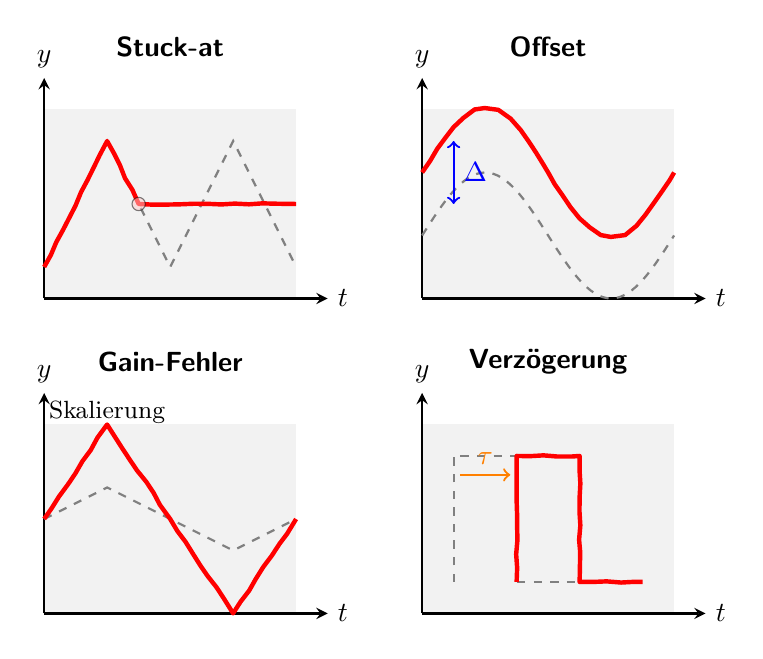
\begin{tikzpicture}[
    scale=0.8,
    % Stil für die Koordinatensysteme
    axis/.style={-stealth, thick},
    % Sollwert-Linie (Referenz)
    soll/.style={gray, dashed, thick},
    % Fehler-Linie (Ist-Wert) mit leichtem Comic-Look
    fault/.style={red, ultra thick, line join=round, decorate, 
                 decoration={random steps, segment length=5pt, amplitude=0.3pt}},
    % Beschriftung
    title/.style={font=\sffamily\bfseries, node distance=0.5cm}
]

% Gitter-Layout Parameter
\def\dx{6}
\def\dy{5}

% --- OBEN LINKS: STUCK-AT ---
\begin{scope}[shift={(0,\dy)}]
    \fill[gray!10] (0,0) rectangle (4,3); % Comic-Schattierung Hintergrund
    \draw[axis] (0,0) -- (4.5,0) node[right] {$t$};
    \draw[axis] (0,0) -- (0,3.5) node[above] {$y$};
    \node[title] at (2,4) {Stuck-at};
    
    \draw[soll] (0,0.5) -- (1,2.5) -- (2,0.5) -- (3,2.5) -- (4,0.5);
    \draw[fault] (0,0.5) -- (1,2.5) -- (1.5,1.5) -- (4,1.5); % Bleibt hängen
    \draw[fill=red!20, opacity=0.5] (1.5,1.5) circle (3pt);
\end{scope}

% --- OBEN RECHTS: OFFSET ---
\begin{scope}[shift={(\dx,\dy)}]
    \fill[gray!10] (0,0) rectangle (4,3);
    \draw[axis] (0,0) -- (4.5,0) node[right] {$t$};
    \draw[axis] (0,0) -- (0,3.5) node[above] {$y$};
    \node[title] at (2,4) {Offset};
    
    \draw[soll] (0,1) sin (1,2) cos (2,1) sin (3,0) cos (4,1);
    \draw[fault] (0,2) sin (1,3) cos (2,2) sin (3,1) cos (4,2); % Konstant nach oben verschoben
    \draw[<->, blue, thick] (0.5,1.5) -- (0.5,2.5) node[midway, right] {$\Delta$};
\end{scope}

% --- UNTEN LINKS: GAIN-FEHLER ---
\begin{scope}[shift={(0,0)}]
    \fill[gray!10] (0,0) rectangle (4,3);
    \draw[axis] (0,0) -- (4.5,0) node[right] {$t$};
    \draw[axis] (0,0) -- (0,3.5) node[above] {$y$};
    \node[title] at (2,4) {Gain-Fehler};
    
    \draw[soll] (0,1.5) -- (1,2) -- (2,1.5) -- (3,1) -- (4,1.5);
    \draw[fault] (0,1.5) -- (1,3) -- (2,1.5) -- (3,0) -- (4,1.5); % Verstärkte Amplitude
    \node at (1,3.2) {\small Skalierung};
\end{scope}

% --- UNTEN RECHTS: VERZÖGERUNG ---
\begin{scope}[shift={(\dx,0)}]
    \fill[gray!10] (0,0) rectangle (4,3);
    \draw[axis] (0,0) -- (4.5,0) node[right] {$t$};
    \draw[axis] (0,0) -- (0,3.5) node[above] {$y$};
    \node[title] at (2,4) {Verzögerung};
    
    \draw[soll] (0.5,0.5) -- (0.5,2.5) -- (1.5,2.5) -- (1.5,0.5) -- (2.5,0.5);
    \draw[fault] (1.5,0.5) -- (1.5,2.5) -- (2.5,2.5) -- (2.5,0.5) -- (3.5,0.5); % Zeitversetzt
    \draw[->, orange, thick] (0.6,2.2) -- (1.4,2.2) node[midway, above] {$\tau$};
\end{scope}

\end{tikzpicture}
\end{document}